\documentclass[10pt,conference]{IEEEtran}
\IEEEoverridecommandlockouts

\usepackage[utf8]{inputenc}
\usepackage[T1]{fontenc}
\usepackage[brazilian]{babel}
\usepackage{cite}
\usepackage{amsmath,amssymb,amsfonts}
\usepackage{graphicx}
\usepackage{textcomp}
\usepackage{xcolor}
\usepackage{booktabs}
\usepackage{url}
\usepackage{balance}

\begin{document}

\title{Para Onde Migra a Atenção dos Desenvolvedores no Stack Web3?\\
Evidência Preliminar a Partir de Repositórios Provider}

\author{\IEEEauthorblockN{Pamella Soares}
\IEEEauthorblockA{Universidade Estadual do Ceará (UECE)\\
Fortaleza, Brasil\\
pamella.soares@aluno.uece.br}
}

\maketitle

\begin{abstract}
Estudos empíricos em software Web3 frequentemente tratam o ecossistema como um domínio relativamente homogêneo, ou concentram-se em fatias específicas (p.ex., plataformas BaaS). Neste \emph{work-in-progress}, provocamos essa premissa: a \textbf{atenção observável dos desenvolvedores}---medida por Issues e Pull Requests em repositórios \emph{provider} do Web3BlockSet---\textbf{migra entre camadas do stack}, alterando ranks e a composição do que é ``Web3'' em cada período. Usamos exclusivamente categorias de repositório \emph{já validadas} (sem classificar a community). Em $\approx$361k documentos (2018--2025, 378 repositórios, 33 categorias), observamos mobilidade relevante de rank (p.ex., \emph{Development Platform} e \emph{Wallet} sobem; \emph{Storage} e \emph{Security Tool} caem), enquanto a concentração top-3 \emph{diminui} (52\%$\rightarrow$45\%). A ideia---ainda em formação---é que o alvo empírico é móvel mesmo quando o domínio parece ``mais diverso''.
\end{abstract}

\begin{IEEEkeywords}
Mining Software Repositories, Web3, atenção de desenvolvedores, evolução de ecossistemas, work-in-progress
\end{IEEEkeywords}

\section{Introdução e Provocação}

O desenvolvimento Web3 é frequentemente descrito como um ecossistema amplo---protocolos, carteiras, DeFi, SDKs, segurança, educação---porém análises empíricas ainda tendem a (i)~agregar fenômenos heterogêneos sob o rótulo ``blockchain/Web3'', ou (ii)~estudar nichos com grande profundidade (p.ex., experiência de desenvolvedores em BaaS~\cite{soares2025bcdex}). Ambas as estratégias são úteis, mas deixam em aberto uma questão \emph{thought-provoking}:

\begin{quote}
\emph{Se a atenção dos desenvolvedores migra entre camadas do stack, conclusões que assumem estabilidade composicional do domínio podem envelhecer rápido---ou generalizar mal.}
\end{quote}

Esta nota short \textbf{não} pretende fechar essa discussão. Seu papel, nos termos do MSR para \emph{work-in-progress papers}, é \textbf{colocar a provocação com evidência preliminar suficiente} para ser discutida, não com a avaliação completa exigida de um full paper.

Concretamente, perguntamos:

\begin{itemize}
\item \textbf{RQ:} Como a atenção de desenvolvimento (Issues/PRs) se redistribui entre categorias validadas de repositórios \emph{provider} no Web3BlockSet entre 2018 e 2025?
\end{itemize}

\paragraph{Por que isto é WIP.}
Não testamos causalidade, não modelamos tópicos de ``dores'', não aplicamos SPACE/BcDEx e não usamos a fatia community (cujas categorias de repositório não foram validadas com o mesmo rigor). A contribuição é uma \emph{ideia controversa/interessante} sustentada por mineração descritiva replicável: mostrar que a composição anual do stack observável muda, e que a hierarquia de longo prazo também se desloca.

\section{Trabalho Relacionado (posicionamento breve)}

Estudos em repositórios blockchain têm caracterizado colaboração e tipos de projetos~\cite{das2022blockchain}, tipologias de issues~\cite{opu2025issuetypes} e desafios de BOSE~\cite{porru2017bose}. O Web3BlockSet~\cite{soares2026web3blockset} oferece categorias de repositório validadas e a dualidade provider/community. Em paralelo, análises de BcDEx em BaaS~\cite{soares2025bcdex} aprofundam tópicos e produtividade em um recorte de plataformas. Este WIP \textbf{não} replica essa linha: em vez de perguntar \emph{quais desafios} dominam, pergunta \emph{para qual camada do stack a atenção migra} ao longo do tempo, usando apenas providers e categorias já validadas. Assim, evitamos sobreposição de contribuição e exploramos uma provocação ortogonal sobre estabilidade composicional do domínio.

\section{Dados e Método (deliberadamente limitado)}

\subsection{Corpus}
Utilizamos o Web3BlockSet~\cite{soares2026web3blockset}, restringindo-nos a documentos com \texttt{data\_source=provider} e \texttt{repository\_category} não vazia (preenchida a partir dos metadados validados dos 381 repositórios oficiais quando o campo no Issue/PR estava ausente). A janela analítica é 2018--2025, resultando em $\approx$361\,071 Issues/PRs, 378 repositórios e 33 categorias. A unidade é o documento Issue/PR; a atenção de uma categoria $c$ no ano $t$ é o volume (e o share) de documentos em repositórios classificados como $c$.

\subsection{Métricas}
(1)~\textbf{Share anual} por categoria (composição do stack observável); (2)~\textbf{concentração} via share das top-3 categorias e índice Herfindahl--Hirschman (HHI) sobre o vetor de shares; (3)~\textbf{mobilidade de rank} das categorias entre 2018 e 2025 ($\Delta$rank $= \mathrm{rank}_{2018}-\mathrm{rank}_{2025}$, positivo se a categoria subiu). Visualmente, o miolo é um \emph{bump chart} (rank ano a ano); o fecho é o $\Delta$rank de longo prazo. Scripts e tabelas estão em \texttt{2027\_short\_paper/}.

\subsection{Validação manual (em andamento)}
Como as categorias já foram validadas no dataset original (acordo global 92,4\% entre especialistas~\cite{soares2026web3blockset}), a amostra cega estratificada por categoria (\texttt{data/manual\_review/}, $n{=}310$) \textbf{não} relabela o stack: ela avalia se o documento é um proxy plausível de \emph{atenção de desenvolvimento} (vs.\ ruído). O protocolo está em \texttt{PROTOCOL\_MANUAL\_REVIEW.md}. Neste WIP reportamos o desenho; percentuais finais de precisão do construto serão incorporados após dupla anotação.

\subsection{O que conscientemente não fazemos}
Não repetimos topic modeling de desafios provider vs.\ community em BaaS~\cite{soares2025bcdex}; não inferimos categorias para a community; não tratamos volume de Issues como satisfação, produtividade ou adoção efetiva de dependências.

\section{Evidência Preliminar}

\subsection{Miolo: composição ano a ano (2018--2025)}
A Figura~\ref{fig:bump} é o eixo do argumento. Um \emph{bump chart} mostra, para cada ano, a posição relativa (rank) das categorias que em algum momento entram no top-5 de atenção. Cruzamentos de linhas significam troca de protagonismo: o ``centro'' do stack provider \emph{não é o mesmo} em 2018, 2021 ou 2025.

\begin{figure}[t]
\centering
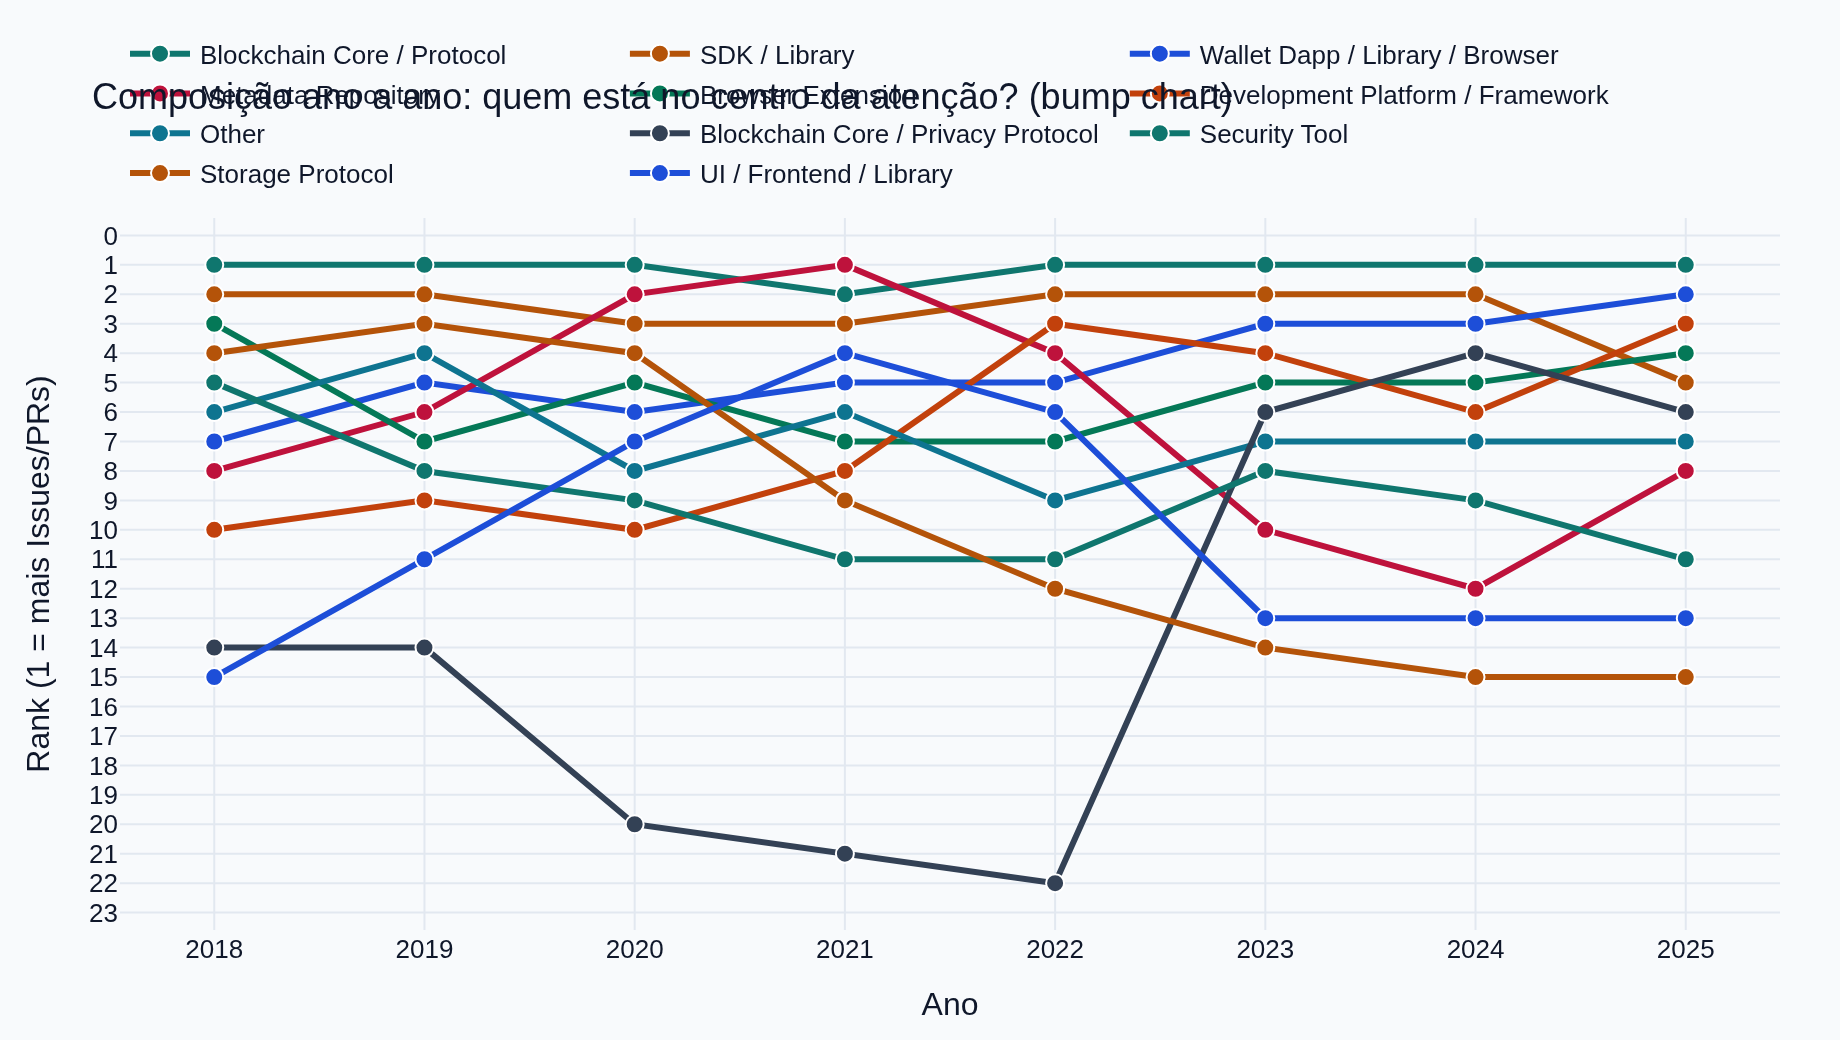
\includegraphics[width=\columnwidth]{figures/fig1_yearly_bump.png}
\caption{Bump chart da atenção provider (2018--2025): rank anual por categoria validada (1~=~mais Issues/PRs). Categorias que entram no top-5 em ao menos um ano.}
\label{fig:bump}
\end{figure}

\paragraph{Leitura em fases.}
\begin{itemize}
\item \textbf{2018--2020:} \emph{Blockchain Core / Protocol} domina (35\%$\rightarrow$41\% do volume anual) e a concentração sobe (top-3 share até $\approx$0,58; HHI até $\approx$0,20).
\item \textbf{2021:} ruptura aparente---\emph{Metadata Repository} salta para $\approx$26\% do volume (rank~1 naquele ano). Tratamos como ano atípico a investigar (monorepos, campanhas, artefatos de coleta), não como tendência estrutural isolada.
\item \textbf{2022--2025:} Core permanece relevante, porém \emph{Wallet} e \emph{Development Platform / Framework} entram de forma estável no topo; a concentração recua e estabiliza (top-3 $\approx$0,42--0,45; HHI $\approx$0,10).
\end{itemize}

A Figura~\ref{fig:conc} sintetiza a concentração; a Figura~\ref{fig:share} mostra shares das principais categorias em área empilhada, reforçando que a \emph{composição} muda mesmo quando o volume total cresce e depois estabiliza ($\approx$25k docs em 2018 para $\approx$57k/ano em 2023--2025).

\begin{figure}[t]
\centering
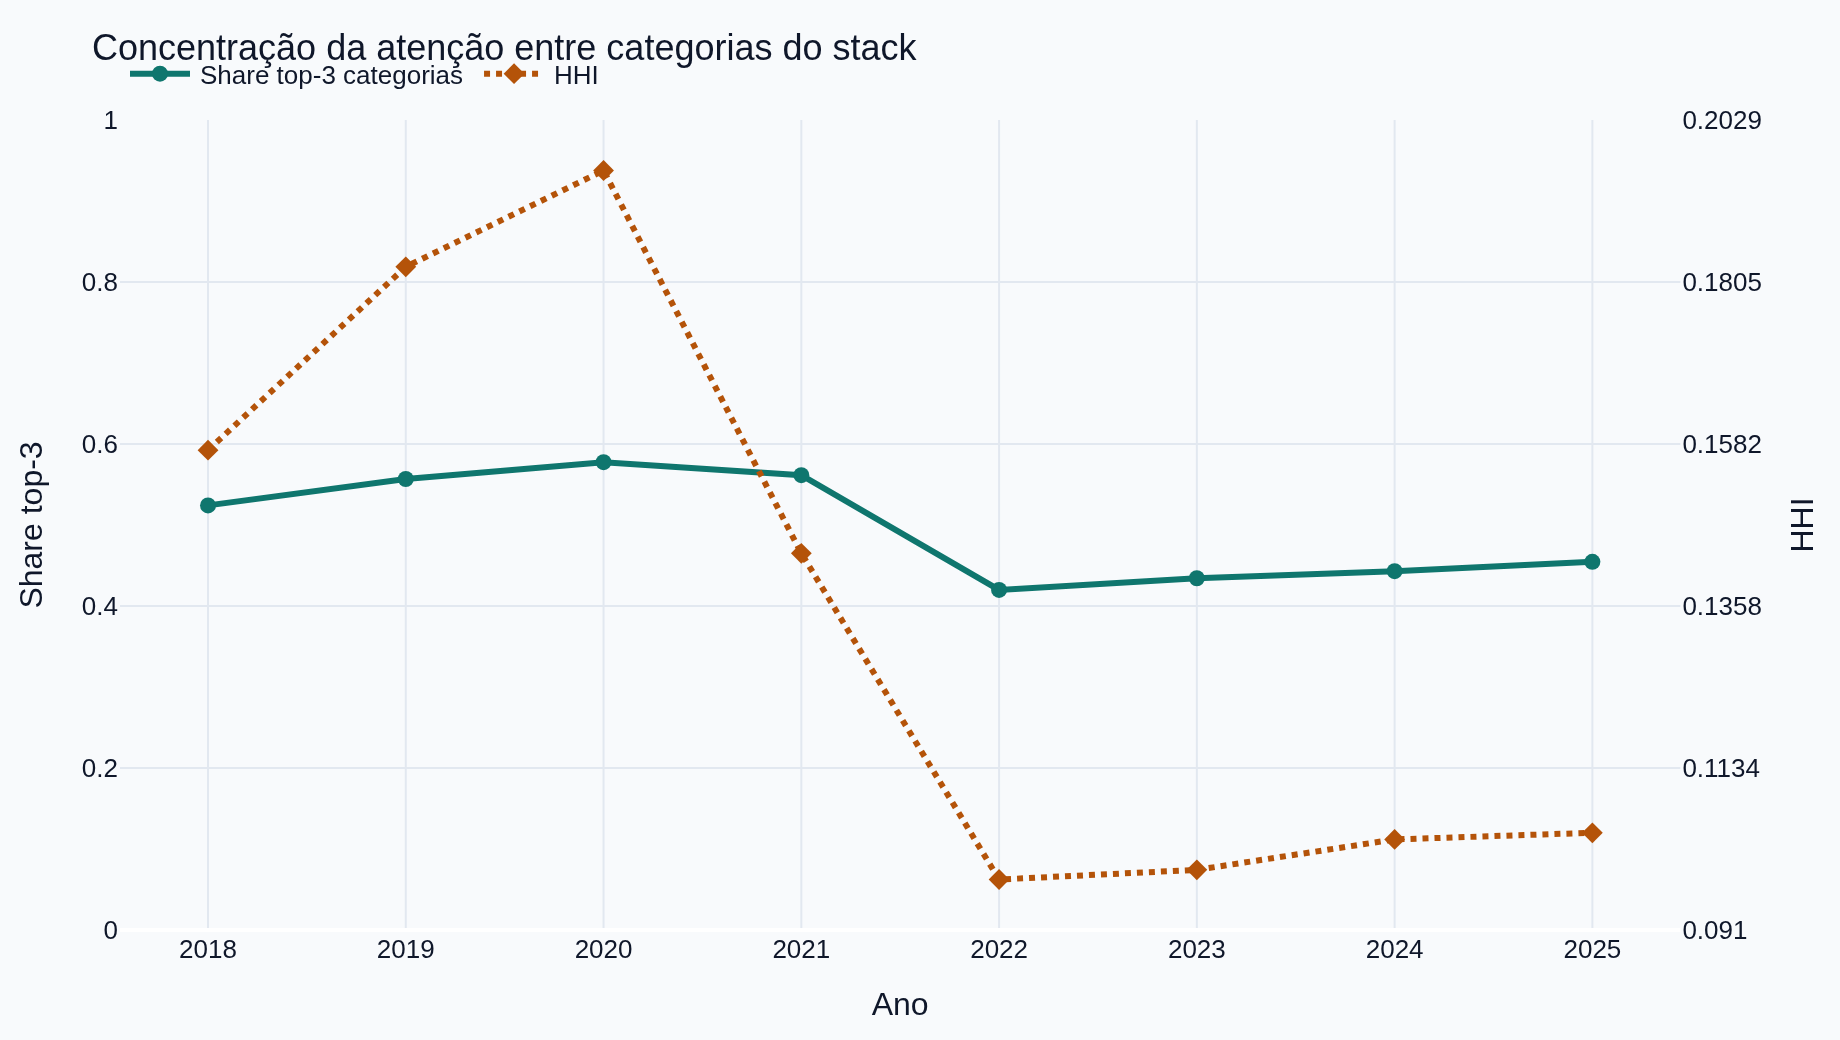
\includegraphics[width=\columnwidth]{figures/fig3_concentration.png}
\caption{Concentração ano a ano: share das top-3 categorias e HHI.}
\label{fig:conc}
\end{figure}

\begin{figure}[t]
\centering
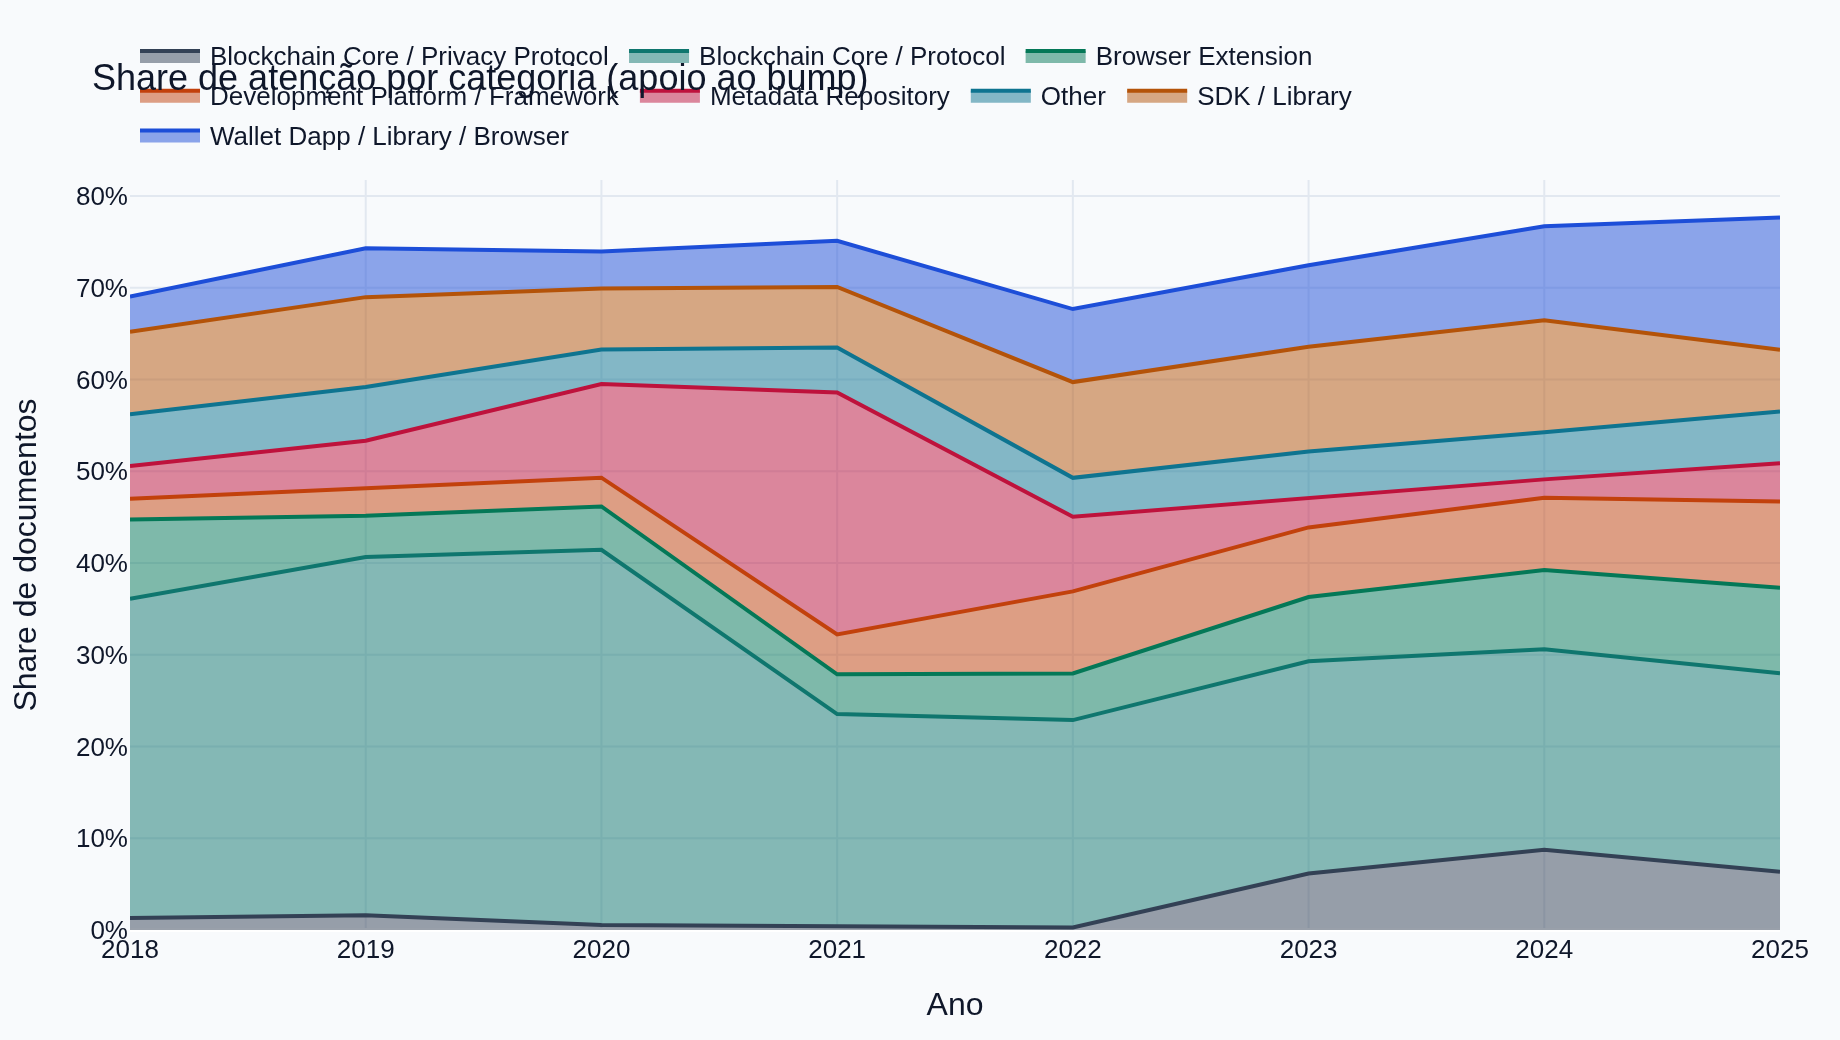
\includegraphics[width=\columnwidth]{figures/fig2_attention_share.png}
\caption{Share de Issues/PRs por categoria (top categorias por volume total). Apoio visual ao bump chart.}
\label{fig:share}
\end{figure}

\subsection{Fecho: mobilidade 2018$\rightarrow$2025}
A Figura~\ref{fig:mob} resume o deslocamento de longo prazo: sobem \emph{Specification}, \emph{Privacy Protocol}, \emph{Development Platform} e \emph{Wallet}; descem \emph{Storage Protocol}, \emph{Security Tool} e \emph{Indexing}. A provocação fecha assim: \textbf{em cada ano, outra composição; no intervalo, outra hierarquia}. Notavelmente, a concentração \emph{não} explode---o share das top-3 cai de 0,52 para 0,45 e o HHI de 0,16 para 0,10. Ou seja, o stack parece ``mais diverso'' em agregados de concentração, ao mesmo tempo em que \textbf{reconfigura quem está no centro}.

\begin{figure}[t]
\centering
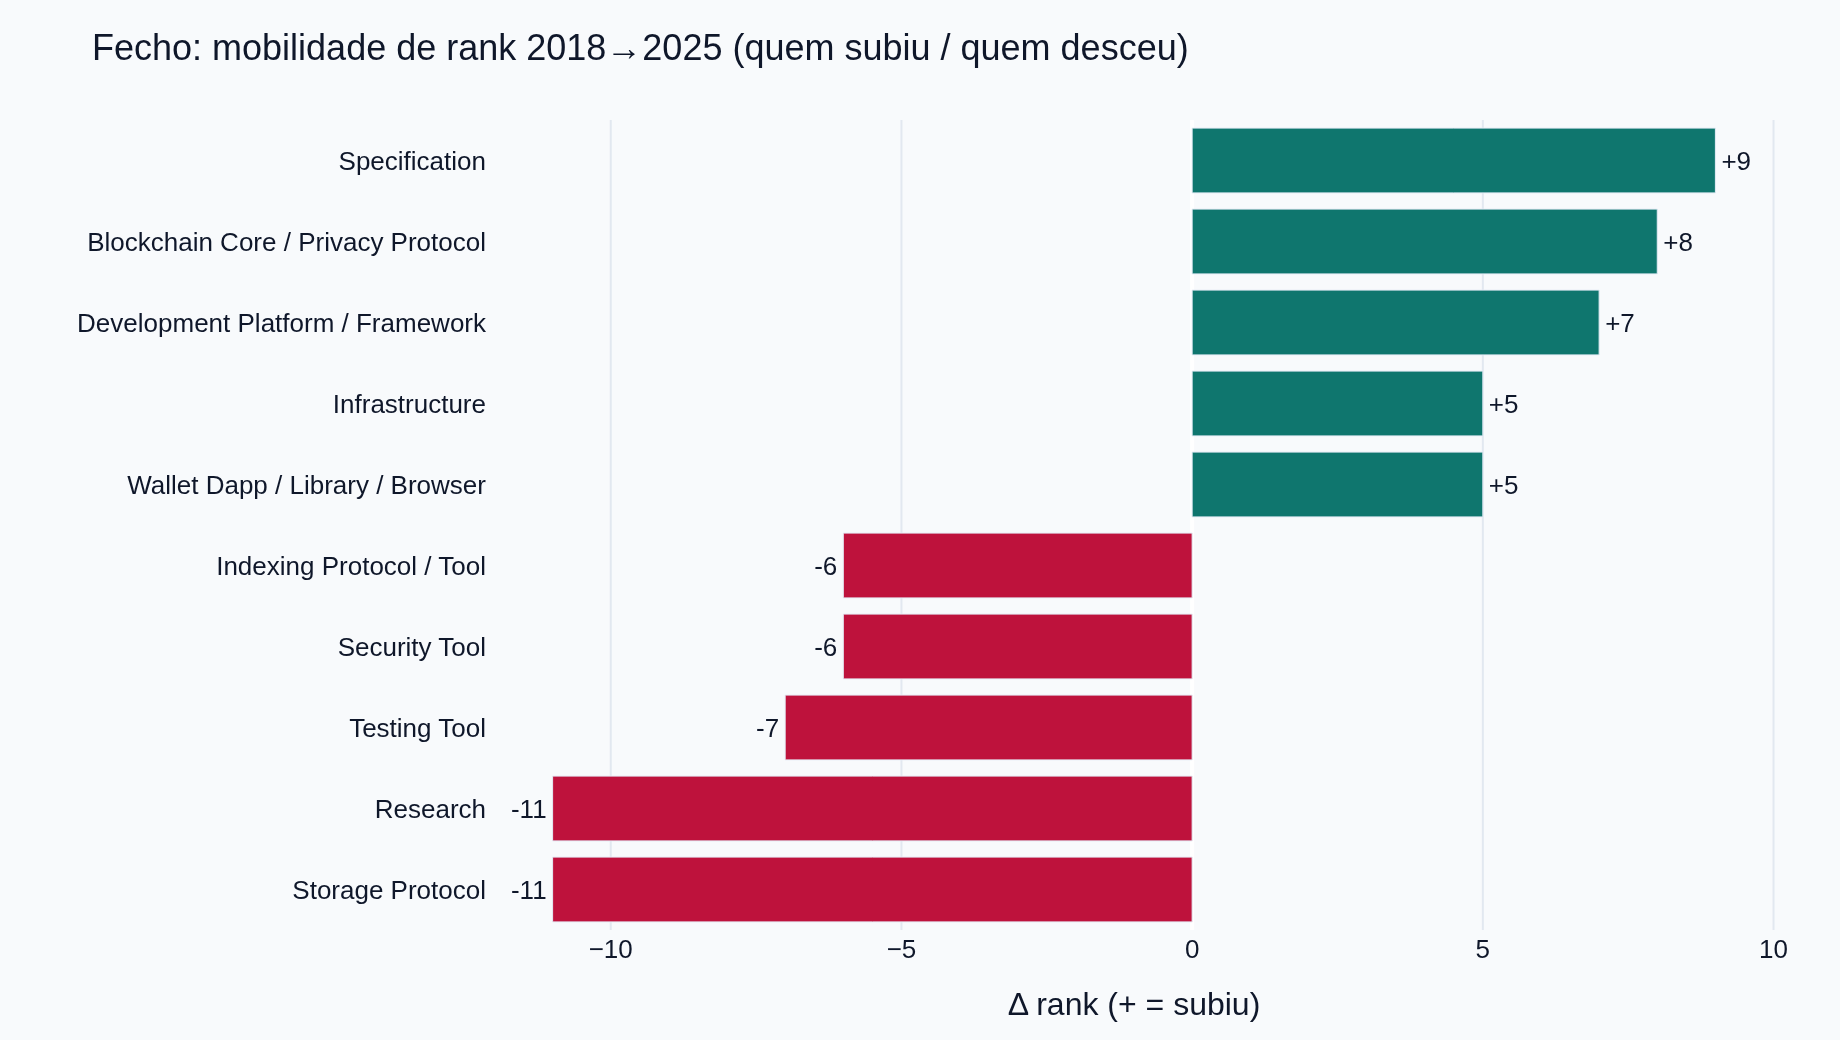
\includegraphics[width=\columnwidth]{figures/fig4_rank_mobility.png}
\caption{Fecho: $\Delta$rank 2018$\rightarrow$2025 (positivos subiram; negativos desceram).}
\label{fig:mob}
\end{figure}

\section{Impacto no ecossistema Web3, atenções e remediações}

\subsection{O que isso implica na prática}
\begin{itemize}
\item \textbf{Pesquisa empírica:} amostrar ``Web3'' num único ano (ou misturar camadas) captura um alvo móvel. Achados sobre desafios, colaboração ou tooling podem ser artefatos da camada quente do período.
\item \textbf{Plataformas e foundations:} roadmaps e DX centrados só em Core/protocol podem subinvestir no que está ganhando atenção (wallets, frameworks, specs).
\item \textbf{Educação e onboarding:} currículos e boilerplates alinhados a um retrato antigo do stack formam desenvolvedores para um ecossistema que já se reconfigurou.
\item \textbf{Segurança e risco:} queda de rank de \emph{Security Tool} \emph{não} implica menos risco---pode indicar atenção deslocada; remediação exige monitorar camadas emergentes, não só o volume histórico de tools de segurança.
\item \textbf{Governança OSS:} organizações multi-produto precisam alocar maintainers onde a atenção (e a carga de Issues/PRs) está migrando.
\end{itemize}

\subsection{Atenções (o que \emph{não} concluir cedo demais)}
\begin{itemize}
\item Volume de Issues/PRs $\neq$ importância técnica, qualidade nem adoção community.
\item Repos oficiais misturam manutenção interna e suporte externo.
\item Cobertura do Web3BlockSet (listas \emph{Awesome}) enviesa quais orgs entram.
\item Categorias, embora validadas, são discretizações; fronteiras (p.ex., SDK vs.\ Wallet) são porosas.
\item Um ano atípico (p.ex., 2021) pode refletir campanhas, monorepos ou eventos de mercado---não só ``mudança estrutural''.
\end{itemize}

\subsection{Remediações recomendadas}
\begin{itemize}
\item \textbf{Estratificar sempre} análises Web3 por camada/categoria e por ano (ou janela), reportando composição da amostra.
\item \textbf{Reamostrar longitudinalmente} benchmarks e datasets; versionar conclusões com o período coberto.
\item \textbf{Separar construtos:} atenção (Issues/PRs) $\neq$ adoção (dependências/manifests) $\neq$ risco (vulns/incidentes).
\item \textbf{Para indústria:} painéis \emph{layer-aware} (atenção por categoria ao longo do tempo) para priorizar docs, SDKs e suporte.
\item \textbf{Para este WIP:} validação manual do construto de atenção; depois, trimestres, Issues vs.\ PRs e triangulação com dependências.
\end{itemize}

Esses pontos são intencionalmente controversos e ainda não totalmente desenvolvidos---espaço próprio da trilha short do MSR.

\section{Ameaças à Validade}

\paragraph{Construto.}
Issues/PRs são proxy de atenção observável, não de esforço interno nem de impacto. A validação manual do construto ainda está em andamento.

\paragraph{Interna.}
Mudanças de composição podem ser influenciadas por crescimento desigual de orgs, arquivamento, ou mudanças de processo GitHub---não apenas por ``interesse genuíno'' dos desenvolvedores.

\paragraph{Externa.}
Generalização para community/adopters está fora do escopo; a seleção via listas \emph{Awesome} limita cobertura a projetos relativamente visíveis.

\paragraph{Confiabilidade.}
Categorias foram validadas no dataset, mas fronteiras entre classes permanecem interpretativas; replicação depende do pacote de scripts e da versão fixa dos CSVs.

\section{Próximos Passos}

A partir desta provocação, planejamos:
\begin{enumerate}
\item concluir a dupla anotação cega do construto de atenção e reportar precisão/$\kappa$;
\item decompor atenção em Issues vs.\ PRs e em sinais de manutenção vs.\ suporte;
\item analisar mobilidade em janelas menores (trimestres) e por organização multi-categoria;
\item triangular com redes de dependência / manifests para separar atenção de adoção;
\item contrastar, em estudo futuro separado, sinais community \emph{sem} reutilizar categorias não validadas;
\item evoluir para full paper com hipóteses pré-registradas e testes de robustez (incluindo sensibilidade à exclusão de 2021).
\end{enumerate}

\section{Conclusão}

Este WIP defende uma ideia simples e desconfortável: \textbf{a atenção dos desenvolvedores no stack Web3 se move}. Com evidência preliminar apenas em providers e categorias validadas, argumentamos que a comunidade empírica deve tratar composição do stack como variável de primeira classe---não como pano de fundo estável. O trabalho está propositalmente incompleto; seu valor está em abrir o debate com dados, um gráfico ano a ano da composição, e um caminho claro de aprofundamento.

\section*{Disponibilidade de Dados}
Scripts, tabelas, figuras e protocolo de revisão manual estão no diretório \texttt{2027\_short\_paper} associado a este manuscrito. O dataset-base é o Web3BlockSet~\cite{soares2026web3blockset}. Para submissão double-anonymous, o pacote será depositado de forma anonimizada.

\bibliographystyle{IEEEtran}
\bibliography{references}

\end{document}
